\chapter{IGAを用いたトランプのバックデザイン生成システム}
本章では,本研究で構築したトランプのバックデザイン生成システムについて説明する.

\section{デザインの表現方法}
本システムで生成されるトランプのバックデザインは,図形の組み合わせで表現される.
図形は,三角形,四角形,五角形,円,円弧,扇形,直線,折線,曲線のいずれかである.
ここでの折線とは,複数の線分を接続した図形を表し,
本研究では2~4個の線分からなる折線のみを扱う.以降,$i$個の線分からなる折線を折線($i$)と表記する.
本システムでは,デザインに対称性を持たせずに図形を配置する場合と,点対称性を持たせて図形を配置する場合がある.
非対称のデザインは1~7個の図形,点対称のデザインは1~7個の図形と各図形を点対称に移動した図形から構成される.
また,縁ありのデザインの場合は縁を白く塗る.
トランプのサイズは一般的にポーカーサイズとブリッジサイズの2つがあるが,本研究で生成するデザインの縦横比はポーカーサイズと同程度とし,サイズを縦300ピクセル,横210ピクセルとする.

\subsection{図形の構成要素}
各図形の構成要素を表\ref{sharp_need}に示す.
ここでの開始角度と終了角度とは,円弧や扇型のもととなる円を時計上においたとき,3時の方向から反時計回りに始点まで進んだ角度が開始角度,終点まで進んだ確度が終了角度とする.
したがって,開始確度と終了角度が同じ場合円になる.

% 開始角度と終了角度の単位はラジアンであり,中心点からそれぞれの角度に線分を伸ばす.
% 開始角度の線分から時計回り,または反時計回りに終了角度の線分を結び円弧を表現する.

\begin{table}[htbp]
	\centering
	\caption{図形の構成要素}
	\begin{tabular}{|l|l|c|} \hline
    \multicolumn{1}{|c|}{図形} & \multicolumn{1}{|c|}{構成要素} & \multicolumn{1}{|c|}{要素数}\\ \hline
	三角形& 3つの頂点の座標,塗り,線の太さ,色情報 & 10\\ \hline
    四角形& 4つの頂点の座標,塗り,線の太さ,色情報 & 12\\ \hline
    五角形& 5つの頂点の座標,塗り,線の太さ,色情報 & 14\\ \hline
    円,円弧&中心の座標,塗り,線の太さ,半径,開始角度,終了角度,色情報 & 9 \\ \hline 
    扇形& 中心の座標,塗り,線の太さ,半径,開始角度,終了角度,色情報 & 9 \\ \hline 
    直線 & 始点の座標,終点の座標,塗り,線の太さ,色情報&8\\ \hline
    折線($i$)& 始点の座標,連結部の座標,終点の座標,塗り,線の太さ,色情報 & 14\\ \hline
    曲線& 始点の座標,制御点の座標,終点の座標,塗り,線の太さ,色情報 & 10\\ \hline
	\end{tabular}
	\label{sharp_need}
\end{table}


\section{染色体の設計}
本システムのIGAにおける染色体はデザインを表現しており,遺伝子はデザインを構成する図形の要素を表している.
表\ref{sharp_need}に示した通り,各図形によって構成要素数が違うが,GAでは交叉する際に個体間で遺伝子を交換するため,1つ図形を構成する遺伝子の個数をそろえる必要がある.
したがって,最も構成要素が多い五角形の要素数に,五角形では使われない要素である,半径,円弧の開始角度,円弧の終了角度の3個を加えた17個の遺伝子で1つの図形を表現する.
デザインは最大7種類の図形で構成されるため,合計19×7=119個の遺伝子ですべての図形を表現できる.
また,デザインの特徴を表す遺伝子を2つ加えて,合計121個の遺伝子でデザインを表現する.
% (17$i$−16)~17$i$番目の遺伝子はi番目の図形の構成要素を表し,120~136番目の遺伝子はデザインの特徴を表す.
染色体の構造を図\ref{iga_chrom}に,図形$i$の遺伝子座と表現型および遺伝子の範囲を表\ref{chrom}に示す.
表\ref{chrom}の$j$の範囲は1≦$j$≦5とする.
また,各図形を表す遺伝子の値を表\ref{sharp}に,各色を表す遺伝子の値を表\ref{color}に示す.

\begin{figure}[b!]
    \begin{center}
    \includegraphics[scale=0.60]{image/iga_chrom.eps}
    \caption{染色体の構造}
    \label{iga_chrom}
    \end{center}
\end{figure}


\begin{table}[htbp]
	\centering
	\caption{図形$i$の遺伝子座と表現型と遺伝子の範囲}
	\begin{tabular}{|l|l|l|} \hline
    \multicolumn{1}{|c|}{遺伝子座} & \multicolumn{1}{|c|}{表現型} & \multicolumn{1}{|c|}{遺伝子の範囲}  \\ \hline
	17($i$–1)     & 図形の種類 & 0 ~ 10 \\ \hline
	17($i$–1)+(2$j$–1)   & $x$座標 & 0 ~ 210 \\ \hline
	17($i$–1)+(2$j$)     & $y$座標 & 0 ~ 300  \\ \hline 
    17($i$–1)+11      & 塗りつぶしの有無 & 0 ~ 1  \\ \hline 
    17($i$–1)+12      & 線の太さ & 0 ~ 30  \\ \hline 
    17($i$–1)+13      & 円の半径 & 0 ~ 150  \\ \hline 
    17($i$–1)+14      & 円弧の開始角度 & 0 ~ 360  \\ \hline
    17($i$–1)+15      & 円弧の終了角度 & 0 ~ 360  \\ \hline
    17($i$–1)+16      & 色情報 & 0 ~ 5  \\ \hline
    119    & 点対称性の有無 & 0 ~ 1  \\ \hline
    120      & 縁の有無 & 0 ~ 1  \\ \hline     
	\end{tabular}
	\label{chrom}
\end{table}

\begin{table}[htbp]
	\centering
	\caption{各図形を表す遺伝子の値}
	\begin{tabular}{|c|l|} \hline
    \multicolumn{1}{|c|}{遺伝子} & \multicolumn{1}{|c|}{図形} \\ \hline
	1     & 三角形\\ \hline
	2   & 四角形 \\ \hline
	3     & 円,円弧 \\ \hline 
    4      & 扇形 \\ \hline 
    5      & 直線 \\ \hline 
    6      & 折れ線($2$) \\ \hline 
    7      & 折れ線($3$) \\ \hline
    8      & 折れ線($4$)\\ \hline
    9      & 曲線\\ \hline
    10      & 五角形\\ \hline  
	\end{tabular}
	\label{sharp}
\end{table}

\begin{table}[htbp]
	\centering
    \caption{各色を表す遺伝子の値}
    \begin{tabular}{|c|l|} \hline
        \multicolumn{1}{|c|}{遺伝子} & \multicolumn{1}{|c|}{色情報} \\ \hline
    0   & white \\ \hline
	1     & red\\ \hline
	2   & green \\ \hline
	3     & blue \\ \hline 
    4      & yellow \\ \hline 
    5      & black \\ \hline  
	\end{tabular}
	\label{color}
\end{table}

\section{初期集団の生成}
GAやIGAでの初期集団は無作為に生成されるのが一般的であるが,本システムでは既存のデザインの特徴から初期集団を生成する.
用いる既存のデザインとしては,複数の図形を組み合わせて表現可能であり,マジック,カーディストリーで使用できるものを選んだ.
既存のデザインの名称と製作者を付録Aに記載する.
本システムで生成するバックデザインは7個以下の図形で表現されるため,既存のデザインの表現に8個以上の図形が必要な場合は,より特徴を表している図形を優先して抽出した.
図\ref{index}のような画面で18個の既存のデザインを提示し,好みや,組み込みたい特徴を持つデザインをユーザに複数選択させる.
システムは選択されたデザインの特徴から30個のデザインを生成し初期集団の個体として提示する.
初期集団の個体に好みの個体がない場合,再生成することができる.

\begin{figure}[t]
    \begin{center}
        \centering
        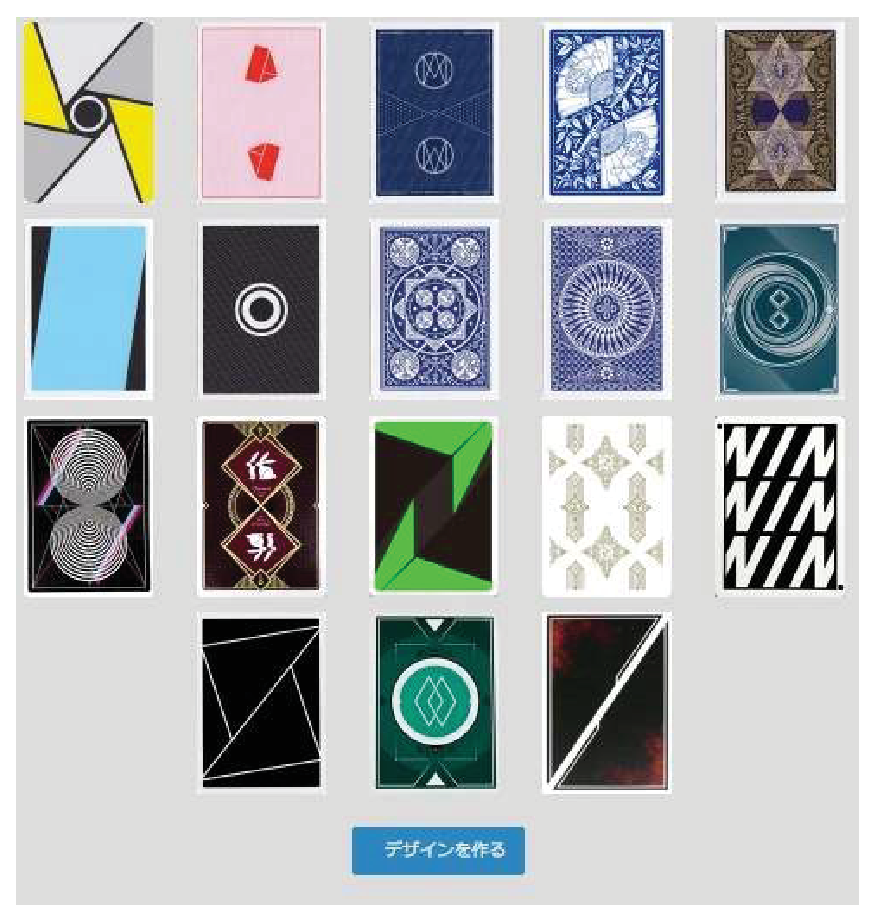
\includegraphics[scale=0.8]{image/index.eps}
        \caption{既存デザインの選択画面}
        \label{index}
    \end{center}
\end{figure}

\section{評価および次世代生成}
評価画面で提示された個体に対して,まったく好みでない場合0点,とても好みの場合5点とする0~5の6段階で評価する.
評価画面を図\ref{value}に示す.
評価値として5点をつけた個体の下には図\ref{elite}のように選択ボタンを表示し,ユーザが特に好みだと感じた場合には,優良デザインとして選択することができる.
優良デザインはすべての過程で合計2つまでとする.
3個以上選択した場合,古いものから削除し,上書きする.
評価値が1点以上の個体とユーザが選択した特に好みの個体から,ルーレット選択を用いて親を選択する.
5点交叉と突然変異率0.5\%の突然変異により次世代の個体を生成する.
突然変異では,遺伝子ごとに格納される数値の範囲が違うため,遺伝子に合わせて数値を変化させる.
突然変異を起こす遺伝子に,図形の種類,色情報,塗りつぶしの有無,点対称性の有無,縁の有無が選ばれた場合,乱数で数値を生成し代入する.
その他の遺伝子が選ばれた場合は,各遺伝子ごとに設定された範囲の乱数を生成する.
各遺伝子ごとの乱数の範囲を表\ref{rand}に示す.
変異前の値を$x$,乱数を$r$,各遺伝子がとりうる数値の上限を$t$としたとき,
$r$が偶数かつ$x$+$r$≦$t$,または$r$が奇数かつ0>$x$–$r$の場合は$x$に$r$を加える.
一方で,$r$が偶数かつ$x$+$r$>$t$,または$r$が奇数かつ0≦$x$–$r$の場合は$x$から$r$を引く.
評価の際にユーザの好みに合わせて背景色,線の色を変更することができる.
色の変更には図\ref{color_picker}のカラーピッカーを用いる.
\label{0404}

% 以上の評価,次世代生成を繰り返し,個体の好みや満足できる個体が得られたとユーザが判断したら処理を終了する.


\begin{figure}[b!]
    \begin{center}
        \centering
        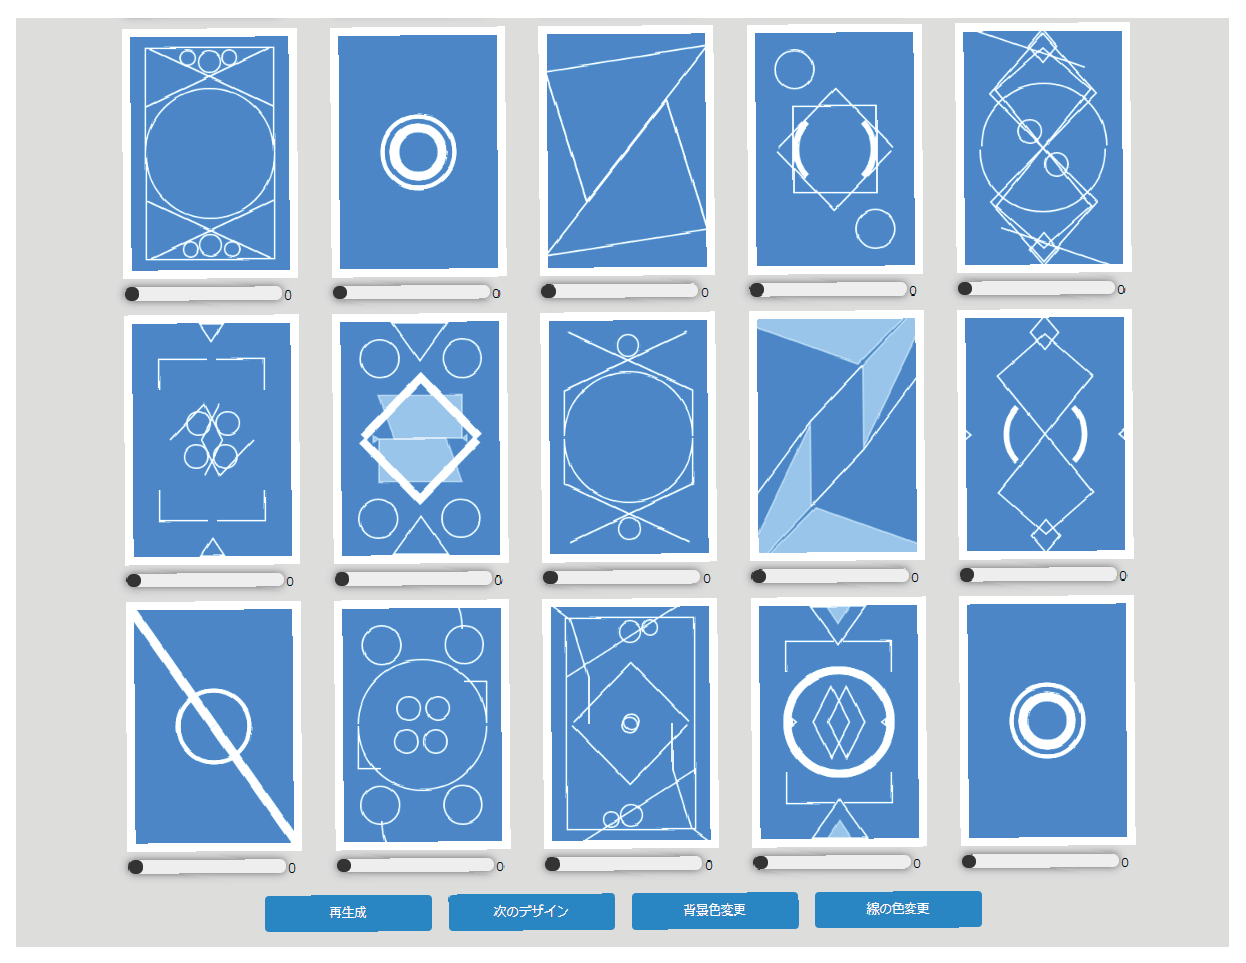
\includegraphics[scale=0.6]{image/value.eps}
        \caption{評価画面}
        \label{value}
    \end{center}
\end{figure}

\begin{figure}[htbp]
    \begin{center}
        \centering
        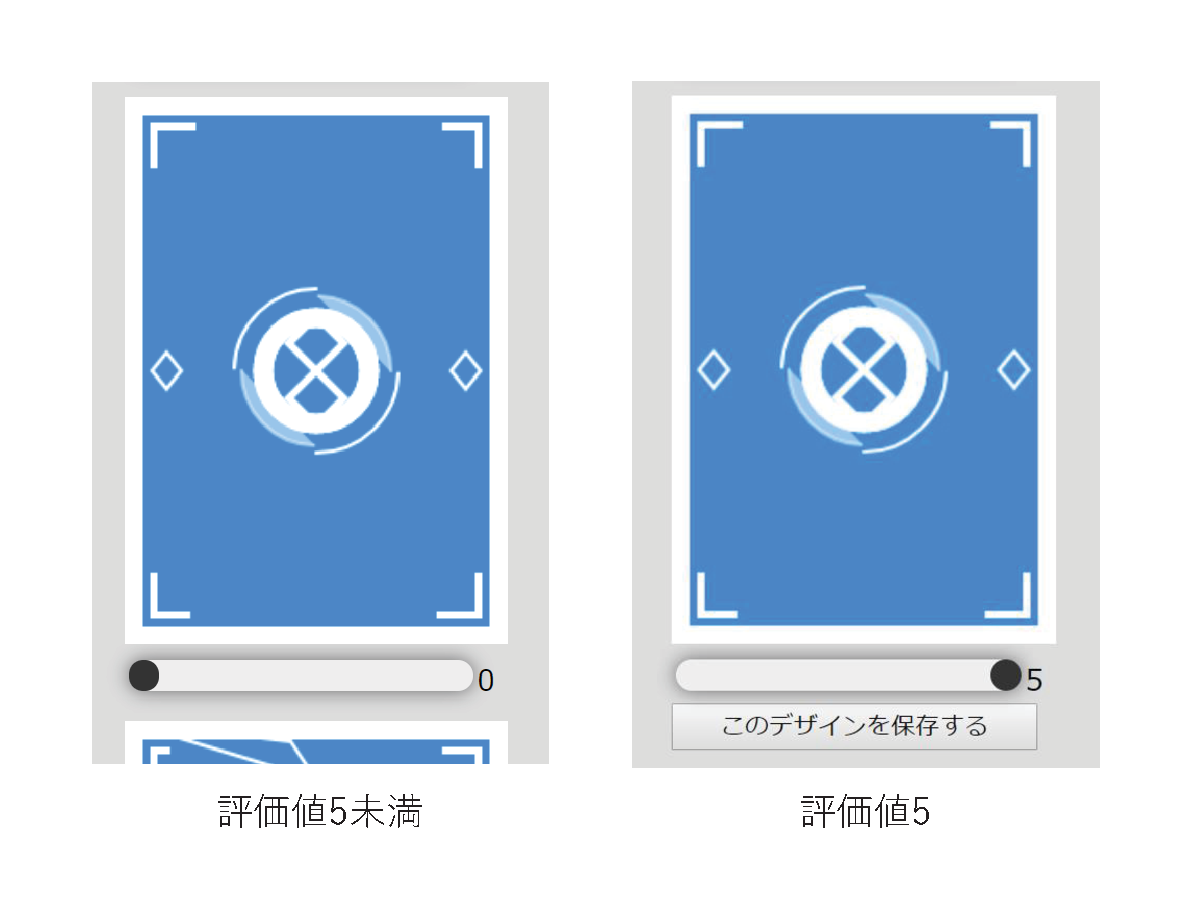
\includegraphics[scale=0.5]{image/value_5.eps}
        \caption{選択ボタン表示の例}
        \label{elite}
    \end{center}
\end{figure}


\begin{figure}[htbp]
    \begin{center}
        \centering
        
\includegraphics[scale=0.5]{image/color_picker.eps}
        \caption{カラーピッカー}
        \label{color_picker}
    \end{center}
\end{figure}

% \subsection{突然変異}
% 本システムのIGAでは,次世代生成の際に0.5\%の確率で突然変異を起こす.
% 遺伝子ごとに格納される数値の範囲が違うので,遺伝子に合わせて数値を変化させる.
% 突然変異する遺伝子に,図形情報,色情報,またはビット数で表されている遺伝子が選ばれた場合,変異前の数値以外を乱数で決め代入する.
% その他の遺伝子が選ばれた場合は,各遺伝子ごとに設定された範囲の乱数を生成する.
% 各遺伝子ごとの乱数の範囲を表\ref{rand}に示す.
% 乱数が奇数だった場合変異前の数値から乱数を引き,偶数だった場合変異前の数値に乱数を加える.
% 乱数が奇数で,変異前の数値が乱数より小さかった場合は乱数を加える処理に変更する.
% 一方,乱数が偶数の際,変異前の数値に乱数を加えると遺伝子に設定された数値の範囲を超える場合,変異前の数値から乱数を引く処理に変更する.

\begin{table}[t]
	\centering
	\caption{表現型と乱数}
	\begin{tabular}{|l|l|} \hline
    \multicolumn{1}{|c|}{表現型}& \multicolumn{1}{|c|}{乱数の範囲} \\ \hline
    $x$座標   & 10~80 \\ \hline
	$y$座標     & 10~80\\ \hline
	線の太さ   & 2~17 \\ \hline
	半径     & 5~35 \\ \hline 
    円弧の開始角度   & 10~110 \\ \hline 
    円弧の終了角度   & 10~110 \\ \hline  
	\end{tabular}
	\label{rand}
\end{table}


\section{終了画面}
評価,次世代生成を繰り返し,個体の好みや満足できる個体が得られたとユーザが判断したら終了画面を表示する.
終了画面では,すべての過程で評価値に4点,5点をつけた個体を高評価個体として表示する.
表示されたデザインをクリックすると,png画像としてダウンロードすることができる.
終了画面を図\ref{last}に示す.
\begin{figure}[htbp]
    \begin{center}
        \centering
        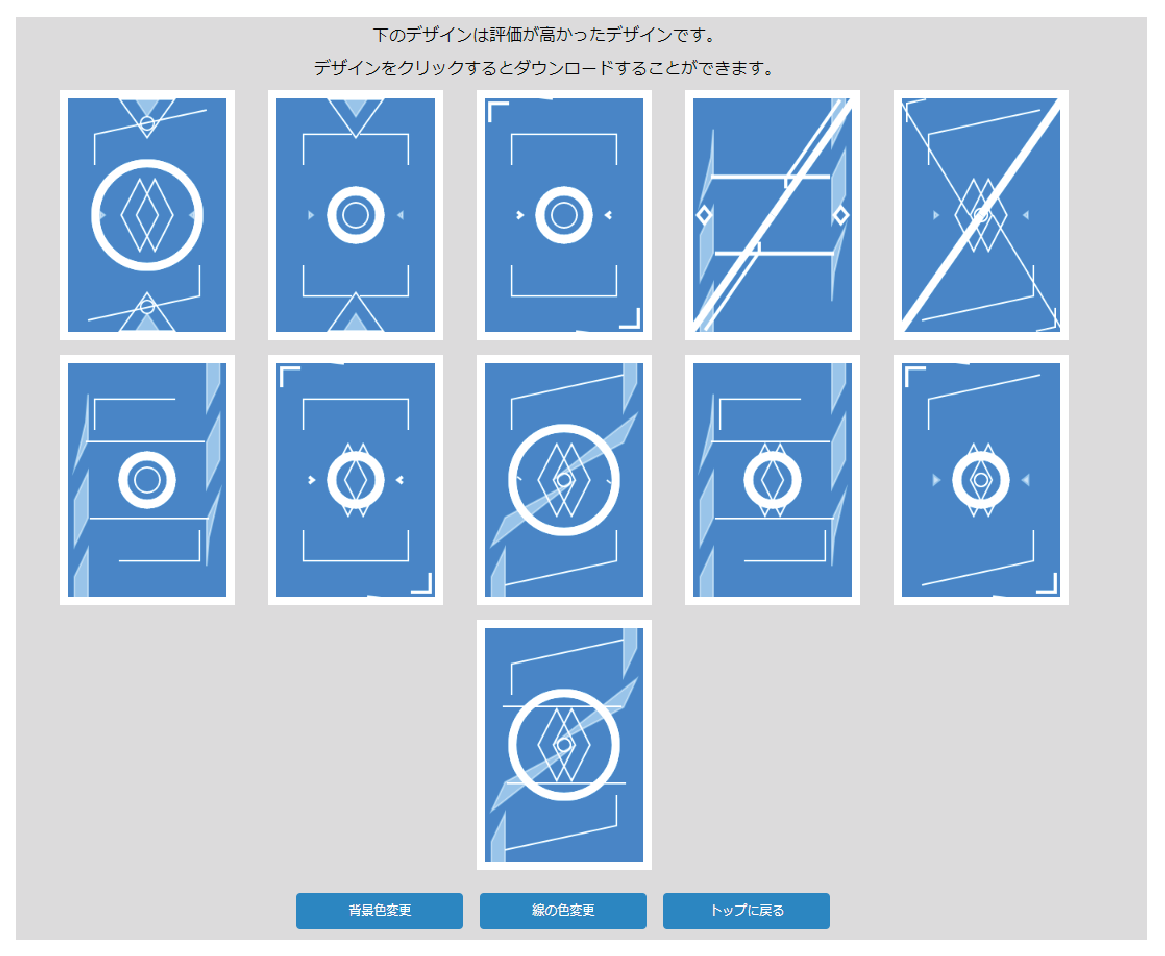
\includegraphics[scale=0.7]{image/last.eps}
        \caption{終了画面}
        \label{last}
    \end{center}
\end{figure}

